
\section{环结构}\label{sec:12-2}

弗洛尔上同调上有一个自然环结构，它由计数三穿孔二球面上的扰动 \BookRecordIndex{T0003}$J$-全纯曲线定义。
把穿孔理解为圆柱端，并如式~\eqref{eq:12-1-3} 那样在穿孔附近作\BookRecordIndex{T0157}哈密顿扰动。更准确地说，
令 $\Sigma$ 为带三个圆柱端的非紧亏格零黎曼曲面，即所谓裤形曲面。假设 $\Sigma$ 上的复
结构在圆柱端上是标准乘积结构。固定圆柱端的参数化
\[
  \phi^\alpha:(-\infty,0)\times\mathbb R/\mathbb Z\longrightarrow\Sigma,
  \qquad
  \phi^\beta,\phi^\gamma:(0,\infty)\times\mathbb R/\mathbb Z\longrightarrow\Sigma,
\]
它们的像互不相交，记
$U^\alpha:=\operatorname{im}\phi^\alpha$、
$U^\beta:=\operatorname{im}\phi^\beta$、
$U^\gamma:=\operatorname{im}\phi^\gamma$。假设补集
\[
  \Sigma'=\Sigma\setminus(U^\alpha\cup U^\beta\cup U^\gamma)
\]
微分同胚于挖去三个开圆盘的二球面；特别地，$\Sigma'$ 是紧的。选取 $\Sigma$ 上的复结构，
使它在三个圆柱端上拉回为标准结构 $s+it$。为定义适当的\BookRecordIndex{T0246}模空间，选取三个哈密顿函数
\[
  H^\alpha,H^\beta,H^\gamma:
  \mathbb R\times\mathbb R/\mathbb Z\times M\longrightarrow\mathbb R,
\]
它们在 $|s|\leq\tfrac12$ 时消失，在 $|s|\geq1$ 时与 $s$ 无关。考虑光滑映射
$u:\Sigma\to M$，要求 $u|_{\Sigma'}$ 是 \BookRecordIndex{T0003}$J$-全纯曲线，并且在圆柱端 $U^\alpha$ 上，
复合 $u^\alpha(s,t):=u\circ\phi^\alpha(s,t)$ 满足
\[
  \partial_su^\alpha+J(u^\alpha)
  \bigl(\partial_tu^\alpha-X^\alpha_{s,t}(u^\alpha)\bigr)=0,
\]
其中对所有 $s,t$ 都有 $\iota(X^\alpha_{s,t})\omega=dH^\alpha_{s,t}$；
$u^\beta:=u\circ\phi^\beta$ 与 $u^\gamma:=u\circ\phi^\gamma$ 满足类似方程。

这些方程的每个有限能量解都满足极限条件
\[
\begin{split}
  \lim_{s\to-\infty}u^\alpha(s,t)&=x^\alpha(t),\\
  \lim_{s\to+\infty}u^\beta(s,t)&=x^\beta(t),\\
  \lim_{s\to+\infty}u^\gamma(s,t)&=x^\gamma(t),
\end{split}
\]
其中 $x^\alpha\in\mathcal P(H^\alpha)$、$x^\beta\in\mathcal P(H^\beta)$、
$x^\gamma\in\mathcal P(H^\gamma)$。这里稍微滥用记号，以 $\mathcal P(H^\alpha)$ 表示
哈密顿量 $H^\alpha_{-\infty,t}$ 的周期解，$\beta,\gamma$ 情形亦同。正确同调类中这些解
$u$ 的空间记为
$\mathcal M(\widetilde x^\alpha;\widetilde x^\beta,\widetilde x^\gamma)$
（见图~\ref{fig:12-2-4}），其维数为
\[
\begin{split}
  \dim\mathcal M(\widetilde x^\alpha;\widetilde x^\beta,\widetilde x^\gamma)
  ={}&\mu_{\mathrm{CZ}}(\widetilde x^\alpha,H^\alpha)
  -\mu_{\mathrm{CZ}}(\widetilde x^\beta,H^\beta)\\
  &-\mu_{\mathrm{CZ}}(\widetilde x^\gamma,H^\gamma)-n.
\end{split}
\]
在零维情形，用与上文相同的论证可知解只有有限多个；其带符号的个数记为
$n(\widetilde x^\alpha;\widetilde x^\beta,\widetilde x^\gamma)$。这些数产生
$\Lambda_\omega$-模同态
\[
  \operatorname{CF}^k(H^\beta)\otimes\operatorname{CF}^\ell(H^\gamma)
  \longrightarrow\operatorname{CF}^{k+\ell+n}(H^\alpha),
  \qquad \xi^\beta\otimes\xi^\gamma\longmapsto\xi^\beta*\xi^\gamma.
\]

\begin{figure}[tbp]
\centering
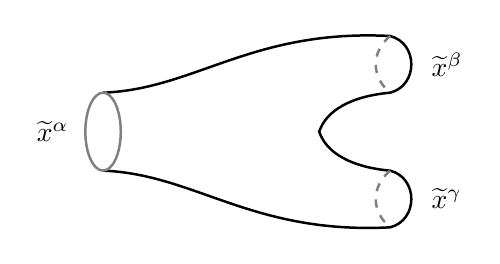
\begin{tikzpicture}[scale=.9]
  \draw[line width=.9pt]
    (-2.6,.55) .. controls (-1.3,.6) and (-.5,1.45) .. (1.45,1.35)
    .. controls (1.85,1.25) and (1.85,.65) .. (1.45,.55)
    .. controls (.9,.5) and (.55,.3) .. (.45,0)
    .. controls (.55,-.3) and (.9,-.5) .. (1.45,-.55)
    .. controls (1.85,-.65) and (1.85,-1.25) .. (1.45,-1.35)
    .. controls (-.5,-1.45) and (-1.3,-.6) .. (-2.6,-.55);
  \draw[gray,line width=.9pt] (-2.6,0) ellipse[x radius=.25,y radius=.55];
  \draw[gray,dashed,line width=.9pt] (1.45,1.35)
    .. controls (1.18,1.12) and (1.18,.78) .. (1.45,.55);
  \draw[gray,dashed,line width=.9pt] (1.45,-.55)
    .. controls (1.18,-.78) and (1.18,-1.12) .. (1.45,-1.35);
  \node[left] at (-2.95,0) {$\widetilde x^\alpha$};
  \node[right] at (1.9,.95) {$\widetilde x^\beta$};
  \node[right] at (1.9,-.95) {$\widetilde x^\gamma$};
\end{tikzpicture}
\caption{\BookRecordIndex{T0217}裤形乘积。}\label{fig:12-2-4}
\end{figure}

它由下式定义：
\[
  (\xi^\beta*\xi^\gamma)(\widetilde x^\alpha):=
  \sum_{\widetilde x^\beta,\widetilde x^\gamma}
  n(\widetilde x^\alpha;\widetilde x^\beta,\widetilde x^\gamma)
  \xi^\beta(\widetilde x^\beta)\xi^\gamma(\widetilde x^\gamma).
\]
\BookRecordIndex{T0132}弗洛尔同调中的通常\BookRecordIndex{T0254}粘合技术表明，此映射是上链同态，因而诱导弗洛尔上同调同态
\[
  \operatorname{HF}^k(H^\beta)\otimes\operatorname{HF}^\ell(H^\gamma)
  \longrightarrow\operatorname{HF}^{k+\ell+n}(H^\alpha).
\]
鉴于其构造，这一映射称为\BookRecordIndex{T0217}裤形乘积，简称 PP 乘积。

\BookRecordIndex{T0132}弗洛尔同调中的通常形变论证表明，\BookRecordIndex{T0217}裤形乘积与定义它时所用黎曼曲面 $\Sigma$ 上的复结构
无关；只要哈密顿函数 $H^\alpha,H^\beta,H^\gamma$ 在 $\pm\infty$ 处不变，它也与这些
函数无关。若在 $\pm\infty$ 处改变它们，再次用弗洛尔\BookRecordIndex{T0254}粘合技术便可证明：此乘积关于
定理~\ref{thm:12-1-3} 的同构是自然的。为在通常符号约定下证明乘积的斜交换性，选取保持
定向的微分同胚 $f:\Sigma\to\Sigma$，交换右侧两个圆柱端。该微分同胚改变 $\Sigma$ 的复
结构，却不影响所得弗洛尔上同调映射。

结合律的证明需要沿一条长圆柱\BookRecordIndex{T0254}粘合两个带三个圆柱端的曲面
$\Sigma_{\alpha;\beta\gamma}$ 与 $\Sigma_{\gamma;\delta\varepsilon}$
（见图~\ref{fig:12-2-5}）。这一过程抵消两个标为 $\gamma$ 的端，得到带四个圆柱端的黎曼
曲面 $\Sigma_{\alpha;\beta\delta\varepsilon}$。若\BookRecordIndex{T0147}颈部充分长，所得三重乘积对应复合
$\xi^\beta*(\xi^\delta*\xi^\varepsilon)$。现在改变
$\Sigma_{\alpha;\beta\delta\varepsilon}$ 上的复结构并以另一种方式分解它，即得
\[
  \xi^\beta*(\xi^\delta*\xi^\varepsilon)
  =(\xi^\beta*\xi^\delta)*\xi^\varepsilon.
\]
这一复结构变化对应于第~\ref{sec:11-1} 节证明\BookRecordIndex{T0229}量子上同调结合律时改变四个\BookRecordIndex{T0150}固定标记点的
\BookRecordIndex{T0185}交比。

\begin{figure}[tbp]
\centering
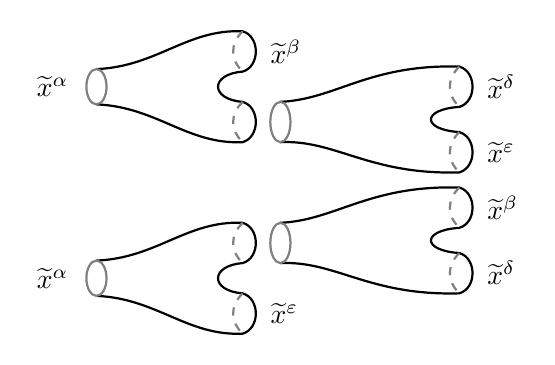
\begin{tikzpicture}[scale=.64,line width=.8pt]
  \draw (-4,2.45) .. controls (-2.8,2.5) and (-2.2,3.25) .. (-1.1,3.2)
    .. controls (-.75,3.1) and (-.75,2.5) .. (-1.1,2.4)
    .. controls (-1.75,2.35) and (-1.75,1.85) .. (-1.1,1.8)
    .. controls (-.75,1.7) and (-.75,1.1) .. (-1.1,1)
    .. controls (-2.2,.95) and (-2.8,1.7) .. (-4,1.75);
  \draw[gray] (-4,2.1) ellipse[x radius=.2,y radius=.35];
  \draw[gray,dashed] (-1.1,3.2) .. controls (-1.35,2.95) and (-1.35,2.65) .. (-1.1,2.4);
  \draw[gray,dashed] (-1.1,1.8) .. controls (-1.35,1.55) and (-1.35,1.25) .. (-1.1,1);
  \draw (-.35,1.8) .. controls (.75,1.85) and (1.4,2.55) .. (3.2,2.5)
    .. controls (3.55,2.4) and (3.55,1.8) .. (3.2,1.7)
    .. controls (2.45,1.65) and (2.45,1.25) .. (3.2,1.2)
    .. controls (3.55,1.1) and (3.55,.5) .. (3.2,.4)
    .. controls (1.4,.35) and (.75,1.05) .. (-.35,1);
  \draw[gray] (-.35,1.4) ellipse[x radius=.2,y radius=.4];
  \draw[gray,dashed] (3.2,2.5) .. controls (2.95,2.25) and (2.95,1.95) .. (3.2,1.7);
  \draw[gray,dashed] (3.2,1.2) .. controls (2.95,.95) and (2.95,.65) .. (3.2,.4);
  \node[left] at (-4.35,2.1) {$\widetilde x^\alpha$};
  \node[right] at (-.75,2.8) {$\widetilde x^\beta$};
  \node[right] at (3.55,2.1) {$\widetilde x^\delta$};
  \node[right] at (3.55,.8) {$\widetilde x^\varepsilon$};

  \draw (-4,-1.35) .. controls (-2.8,-1.3) and (-2.2,-.55) .. (-1.1,-.6)
    .. controls (-.75,-.7) and (-.75,-1.3) .. (-1.1,-1.4)
    .. controls (-1.75,-1.45) and (-1.75,-1.95) .. (-1.1,-2)
    .. controls (-.75,-2.1) and (-.75,-2.7) .. (-1.1,-2.8)
    .. controls (-2.2,-2.85) and (-2.8,-2.1) .. (-4,-2.05);
  \draw[gray] (-4,-1.7) ellipse[x radius=.2,y radius=.35];
  \draw[gray,dashed] (-1.1,-.6) .. controls (-1.35,-.85) and (-1.35,-1.15) .. (-1.1,-1.4);
  \draw[gray,dashed] (-1.1,-2) .. controls (-1.35,-2.25) and (-1.35,-2.55) .. (-1.1,-2.8);
  \draw (-.35,-.6) .. controls (.75,-.55) and (1.4,.15) .. (3.2,.1)
    .. controls (3.55,0) and (3.55,-.6) .. (3.2,-.7)
    .. controls (2.45,-.75) and (2.45,-1.15) .. (3.2,-1.2)
    .. controls (3.55,-1.3) and (3.55,-1.9) .. (3.2,-2)
    .. controls (1.4,-2.05) and (.75,-1.35) .. (-.35,-1.4);
  \draw[gray] (-.35,-1) ellipse[x radius=.2,y radius=.4];
  \draw[gray,dashed] (3.2,.1) .. controls (2.95,-.15) and (2.95,-.45) .. (3.2,-.7);
  \draw[gray,dashed] (3.2,-1.2) .. controls (2.95,-1.45) and (2.95,-1.75) .. (3.2,-2);
  \node[left] at (-4.35,-1.7) {$\widetilde x^\alpha$};
  \node[right] at (3.55,-.3) {$\widetilde x^\beta$};
  \node[right] at (3.55,-1.6) {$\widetilde x^\delta$};
  \node[right] at (-.75,-2.4) {$\widetilde x^\varepsilon$};
\end{tikzpicture}
\caption{结合律。}\label{fig:12-2-5}
\end{figure}

\paragraph{比较定理。}
由定理~\ref{thm:12-1-4}，弗洛尔上同调群 $\operatorname{HF}^*(H,J)$ 自然同构于\BookRecordIndex{T0229}量子
上同调群 $\operatorname{QH}^*(M)$；因而可以预期，在此同构下\BookRecordIndex{T0217}裤形乘积对应于杯积的量子
形变。即使 $\pi_2(M)=0$，即量子形变等于通常杯积时，这个问题也并不平凡。Schwarz
\srcite{358} 在其论文中证明了 $\pi_2(M)=0$ 的情形，Piunikhin--Salamon--Schwarz
\srcite{323} 证明了一般情形。Liu--Tian \srcite{250} 与 Ruan--Tian \srcite{347} 还
各自独立给出了其他证明；Sadov \srcite{350} 给出了物理学家的处理方式。

\begin{theorem}\label{thm:12-2-1}
设 $(M,\omega)$ \BookRecordIndex{T0058}半正，并设
\[
  \Phi^\alpha:\operatorname{HF}^*(M,\omega,H^\alpha,J^\alpha)
  \longrightarrow\operatorname{QH}^*(M)
\]
是定理~\ref{thm:12-1-4} 的 PSS 同构；$\Phi^\beta,\Phi^\gamma$ 类似。则
\[
  \Phi^\alpha(\xi^\beta*\xi^\gamma)
  =\Phi^\beta(\xi^\beta)*\Phi^\gamma(\xi^\gamma)
\]
对 $\xi^\beta\in\operatorname{HF}^*(H^\beta)$ 与
$\xi^\gamma\in\operatorname{HF}^*(H^\gamma)$ 成立。左侧乘积由裤形构造定义，右侧乘积是
杯积的量子形变。
\end{theorem}

证明思路如下。先用 Morse--Witten 复形以一种略微不同的方式表示杯积的量子形变。给定
三个 Morse 函数 $f^\alpha,f^\beta,f^\gamma:M\to\mathbb R$、三个\BookRecordIndex{T0233}临界点
$x^\alpha,x^\beta,x^\gamma$、三个互异点
$w^\alpha,w^\beta,w^\gamma\in\mathbb{CP}^1$，以及定义~\ref{def:6-7-10} 中的正则\BookRecordIndex{T0088}殆复
结构族
\[
  J=\{J_z\}_{z\in S^2}\in
  \mathcal J_{\mathrm{reg}}(S^2;M,\omega;\mathbf w)
\]
（$J_z$ 接近某个固定\BookRecordIndex{T0088}殆复结构 $J_0$），考虑空间
\[
  \mathcal M_A(x^\alpha;x^\beta,x^\gamma)
  =\mathcal M_A(x^\alpha;x^\beta,x^\gamma;f,J),
\]
它由满足
\[
\begin{split}
  u(w^\alpha)&\in W^u(x^\alpha,f^\alpha),\\
  u(w^\beta)&\in W^s(x^\beta,f^\beta),\\
  u(w^\gamma)&\in W^s(x^\gamma,f^\gamma)
\end{split}
\]
的全部 $J$-全纯 $A$-球面 $u:\mathbb{CP}^1\to M$ 组成。
\sourcefootnote{原书从本段开头\BookRecordIndex{T0150}固定标记点 $w^\alpha,w^\beta,w^\gamma$，但随后在\BookRecordIndex{T0246}模空间条件
中改用未定义的 $z^\alpha,z^\beta,z^\gamma$，并把度量下标写成 $J_{z^i}$；这里统一恢复为
$w^\alpha,w^\beta,w^\gamma$ 与 $J_{w^i}$。}
这里 $W^s(x,f)$、$W^u(x,f)$ 表示\BookRecordIndex{T0233}临界点 $x$ 关于 Morse 函数 $f$ 向下梯度流的稳定与
不稳定流形。$f^i$ 的梯度相对于 $J_{w^i}$ 诱导的度量理解，其中
$i=\alpha,\beta,\gamma$；假设这些梯度流为 Morse--Smale。可把
$\mathcal M_A(x^\alpha;x^\beta,x^\gamma)$ 的元素看成带尖部的 $J$-全纯球面
（见图~\ref{fig:12-2-6}）。

\begin{figure}[tbp]
\centering
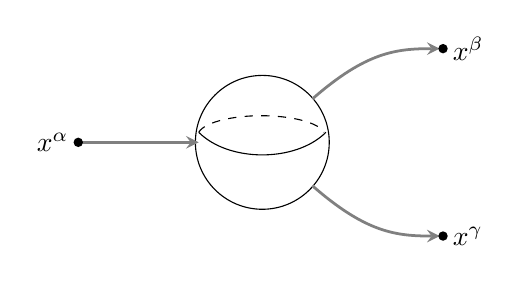
\begin{tikzpicture}[>=stealth,scale=.85]
  \draw (0,0) circle (1);
  \draw[dashed] (-.95,.15) arc[start angle=170,end angle=10,x radius=.95,y radius=.3];
  \draw (-.95,.15) .. controls (-.5,-.3) and (.5,-.3) .. (.95,.15);
  \draw[gray,->,line width=1pt] (-2.7,0)--(-.95,0);
  \draw[gray,->,line width=1pt] (.75,.65)..controls (1.55,1.35) and (2,1.4)..(2.65,1.4);
  \draw[gray,->,line width=1pt] (.75,-.65)..controls (1.55,-1.35) and (2,-1.4)..(2.65,-1.4);
  \fill (-2.75,0) circle (2pt) node[left] {$x^\alpha$};
  \fill (2.7,1.4) circle (2pt) node[right] {$x^\beta$};
  \fill (2.7,-1.4) circle (2pt) node[right] {$x^\gamma$};
\end{tikzpicture}
\caption{通过 Morse 理论得到的量子乘积。}\label{fig:12-2-6}
\end{figure}

由如下维数公式
\sourcefootnote{原书把第二式的不稳定流形误印作 $W^u(x,H)$；此段只涉及 Morse 函数 $f$，
且右端正是 $f$ 的 Morse 指数，故改为 $W^u(x,f)$。}：
\[
  \dim W^s(x,f)=2n-\operatorname{ind}_f(x),\qquad
  \dim W^u(x,f)=\operatorname{ind}_f(x),
\]
对一般的 Morse 函数 $f^\alpha,f^\beta,f^\gamma$，有
\[
  \dim\mathcal M_A(x^\alpha;x^\beta,x^\gamma)
  =2c_1(A)+\operatorname{ind}_{f^\alpha}(x^\alpha)
  -\operatorname{ind}_{f^\beta}(x^\beta)
  -\operatorname{ind}_{f^\gamma}(x^\gamma).
\]
当此维数为零时，把 $\mathcal M_A(x^\alpha;x^\beta,x^\gamma)$ 中按适当符号计数的点数记作
$n_A(x^\alpha;x^\beta,x^\gamma)$。于是得到链映射
\[
  \operatorname{CM}^*(f^\beta;\Lambda_\omega)
  \otimes\operatorname{CM}^*(f^\gamma;\Lambda_\omega)
  \longrightarrow\operatorname{CM}^*(f^\alpha;\Lambda_\omega),
  \qquad \xi^\beta\otimes\xi^\gamma\longmapsto\xi^\beta*\xi^\gamma,
\]
\sourcefootnote{原书在这里把三个 Morse--Witten 复形依次印作
$\operatorname{CF}^*(f^\beta;\Lambda_\omega)$、
$\operatorname{CF}^*(f^\gamma;\Lambda_\omega)$ 与
$C^*(f^\alpha;\Lambda_\omega)$；本节前文已把 Morse 复形统一记为
$\operatorname{CM}^*$，故将三处统一补正。}
其定义为
\begin{equation}\label{eq:12-2-1}
  (\xi^\beta*\xi^\gamma)(x^\alpha,A^\alpha)
  =\sum_{\substack{A,\,x^\beta,\,x^\gamma,\,A^\beta,\,A^\gamma\\
                    A+A^\alpha=A^\beta+A^\gamma}}
  n_A(x^\alpha;x^\beta,x^\gamma)
  \xi^\beta(x^\beta,A^\beta)\xi^\gamma(x^\gamma,A^\gamma).
\end{equation}
\sourcefootnote{原书此式的求和号仅列 $A^\beta+A^\gamma=A^\alpha$，因而把\BookRecordIndex{T0285}球面类 $A$ 与
\BookRecordIndex{T0233}临界点 $x^\beta,x^\gamma$ 留成自由变量，并在同调类约束中漏掉 $A$。紧邻的零维公式与
$\deg(x,A)=\operatorname{ind}_f(x)-2c_1(A)$ 唯一给出
$A+A^\alpha=A^\beta+A^\gamma$；这里也补齐全部求和变量。}
它在 Morse--Witten 上同调（取 $\Lambda_\omega$ 系数，上边缘映射为
$\delta_{\mathrm{MW}}$）上诱导乘积，因而也在\BookRecordIndex{T0229}量子上同调上诱导乘积。这个乘积等于\BookRecordIndex{T0228}量子
杯积，因为 Morse 函数\BookRecordIndex{T0233}临界点的稳定、不稳定流形表示生成 $M$ 上同调的上同调类。

\begin{figure}[tbp]
\centering
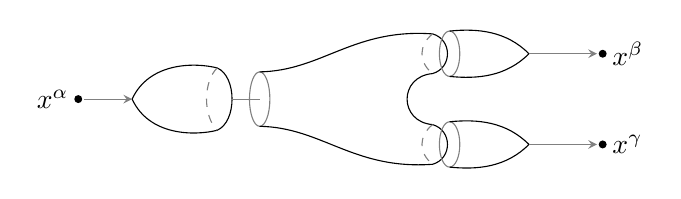
\begin{tikzpicture}[>=stealth,scale=.72]
  \fill (-5,0) circle (2pt) node[left] {$x^\alpha$};
  \draw[gray,->] (-4.9,0)--(-4.05,0);
  \draw (-4.05,0)
    .. controls (-3.75,.65) and (-2.95,.65) .. (-2.55,.55)
    .. controls (-2.2,.4) and (-2.2,-.4) .. (-2.55,-.55)
    .. controls (-2.95,-.65) and (-3.75,-.65) .. (-4.05,0);
  \draw[gray,dashed] (-2.55,.55)
    .. controls (-2.8,.3) and (-2.8,-.3) .. (-2.55,-.55);
  \draw[gray] (-2.3,0)--(-1.8,0);
  \draw[gray] (-1.8,0) ellipse[x radius=.18,y radius=.48];
  \draw (-1.8,.48) .. controls (-.7,.5) and (-.15,1.25) .. (1.25,1.15)
    .. controls (1.6,1.05) and (1.6,.55) .. (1.25,.45)
    .. controls (.65,.4) and (.65,-.4) .. (1.25,-.45)
    .. controls (1.6,-.55) and (1.6,-1.05) .. (1.25,-1.15)
    .. controls (-.15,-1.25) and (-.7,-.5) .. (-1.8,-.48);
  \draw[gray,dashed] (1.25,1.15) .. controls (1, .95) and (1,.65) .. (1.25,.45);
  \draw[gray,dashed] (1.25,-.45) .. controls (1,-.65) and (1,-.95) .. (1.25,-1.15);
  \draw[gray] (1.55,.8) ellipse[x radius=.18,y radius=.4];
  \draw[gray] (1.55,-.8) ellipse[x radius=.18,y radius=.4];
  \draw (1.55,1.2) .. controls (2.05,1.25) and (2.55,1.2) .. (2.95,.8)
    .. controls (2.55,.4) and (2.05,.35) .. (1.55,.4);
  \draw (1.55,-.4) .. controls (2.05,-.35) and (2.55,-.4) .. (2.95,-.8)
    .. controls (2.55,-1.2) and (2.05,-1.25) .. (1.55,-1.2);
  \draw[gray,->] (2.95,.8)--(4.15,.8);
  \draw[gray,->] (2.95,-.8)--(4.15,-.8);
  \fill (4.25,.8) circle (2pt) node[right] {$x^\beta$};
  \fill (4.25,-.8) circle (2pt) node[right] {$x^\gamma$};
\end{tikzpicture}
\caption{\BookRecordIndex{T0229}量子上同调与\BookRecordIndex{T0217}裤形乘积。}\label{fig:12-2-7}
\end{figure}

现在由\BookRecordIndex{T0132}弗洛尔同调中的标准\BookRecordIndex{T0254}粘合论证可知，定理~\ref{thm:12-1-4} 的 PSS 同构
\[
  \Phi^\alpha:\operatorname{HF}^*(H^\alpha)
  \longrightarrow\operatorname{QH}^*(M;\Lambda_\omega)
\]
按照 \srcite{323} 的描述交织这两种乘积结构。要看出这一点，须把三个 $J$-全纯\BookRecordIndex{T0182}尖盘粘到
一条 $J$-全纯裤形曲线的边界上。更准确地说，边界分支是邻接周期解的圆柱端，\BookRecordIndex{T0254}粘合时使用
弗洛尔\BookRecordIndex{T0256}粘合定理。结果得到上文所述带三个尖部的（扰动）$J$-全纯球面
（见图~\ref{fig:12-2-7}）。论证的更多细节见 \srcite{323}。注意，
定理~\ref{thm:12-2-1} 还给出了量子乘积结合律的另一个证明。
